% =============================================================================
% Zero-skipping 3x3 convolution engine on a Spartan-7 FPGA
% Manuscript v5 (IEEEtran, journal mode, guaranteed single column)
%
% POLICY OF THIS FILE
%  * Format: IEEEtran journal mode, single column [11pt,journal,draftclsnofoot,onecolumn].
%    NOTE: In IEEEtran.cls, the 'onecolumn' option is ignored in final journal mode
%    unless 'draftclsnofoot' (or draftcls) is specified. draftclsnofoot provides
%    clean single-column journal layout without draft footers.
%  * Every number comes from verified project run files (final verified run
%    results/final_run_20261030_1056, funcsim_v2, SAIF flow v2, and board_results
%    master silicon benchmark) or is a stated arithmetic consequence of those numbers.
%  * Anything not yet measured is marked with \todo{...} (red, bold).
%  * FPGA validation data is strictly tagged [BOARD-MEASURED] (compute cycles, skip counts,
%    wall-clock execution time over UART, bit-exact comparisons).
%  * No power or energy claims are made from board data; all energy figures are SAIF
%    tool estimates and explicitly stated as such.
%  * Reference list: numbered in order of first citation. Entries carrying
%    a "% VERIFY" comment were found by search but one detail is still to be
%    checked against the publisher record.
%  * Terminology strictly follows guidelines: "FPGA validation", "clock-enable (CE) gating",
%    "estimated Fmax from WNS at 50 MHz", and "tool estimate" for SAIF energy.
% =============================================================================
\documentclass[11pt,journal,draftclsnofoot,onecolumn]{IEEEtran}

\usepackage{amsmath,amssymb}
\usepackage{graphicx}
\usepackage{booktabs}
\usepackage{array}
\usepackage{cite}
\usepackage{xcolor}
\usepackage{algorithm}
\usepackage{algpseudocode}
\usepackage{pgfplots}
\pgfplotsset{compat=1.16}

% Standard journal line spacing (not double-spaced draft)
\linespread{1.15}

% ---- helpers ----------------------------------------------------------------
\newcommand{\todo}[1]{\textbf{\textcolor{red}{[TO COMPLETE: #1]}}}
% Insert a figure if the file exists, otherwise a visible placeholder box.
\newcommand{\figorbox}[3]{%
  \IfFileExists{#1}{\includegraphics[width=#2]{#1}}%
  {\fbox{\parbox{#2}{\centering\small\textcolor{red}{Figure file \texttt{\detokenize{#1}} missing}\\[2pt]#3}}}}

\begin{document}

\title{A Zero-Skipping Serial MAC Engine for 3$\times$3 Convolution on a Spartan-7 FPGA: Ablation, Cycle and Energy Evaluation}

\author{Krutadnya~Bodake, Anushka~Shinde, and~Pranav~Raypelli%
\thanks{The authors are with the Department of Electronics and Computer Science (EXCS), Vidyalankar Institute of Technology, Mumbai 400037, India (e-mail: krutadnya.bodake@vit.edu.in; anushka.shinde@vit.edu.in; pranav.raypelli@vit.edu.in).}}

\maketitle

% =============================================================================
\begin{abstract}
A serial multiply-accumulate (MAC) engine normally spends one clock cycle on every
kernel tap, even when the product is zero. We built a serial 3$\times$3 convolution
engine for an AMD/Xilinx Spartan-7 XC7S15 FPGA at 50~MHz with three optional mechanisms:
priority-encoded zero-skipping (ZS), operand isolation (OI), and accumulator
clock-enable (CE) gating (CG). All eight combinations were implemented from one top level,
together with a static schedule that skips only the three known-zero taps of the
Sobel-X kernel. Every engine matched a golden model with zero output mismatches in RTL
simulation, and all nine matched in zero-delay gate-level simulation of the routed
netlists. On Sobel-X filtering of real images, ZS reduced the measured start-to-done
latency from 11 to 7.89 cycles per patch ($1.39\times$); the static schedule alone
reached $1.375\times$, so run-time zero detection added only 1.4\,\%. With dense kernels,
ZS never took more cycles than the baseline, and on ReLU activation maps of 14 images its
speedup was $1.78\times$ to $4.18\times$ (median $2.01\times$). Operand isolation
synthesized to nothing when combined with CG or ZS, and CG alone gave no resolvable
energy change. SAIF-based power estimates, which are tool estimates and not board
measurements, put the energy per patch of the static schedule 31.6\,\% below the baseline
on Sobel-X, ZS 8.7\,\% below, and ZS 36.5\,\% below on a dense-kernel ReLU workload.
Physical FPGA validation was executed across all nine bitstreams on an Invent Logics
EDGE Spartan-7 board over physical USB-UART, processing 298{,}368 physical patches across
a 3-image benchmark suite ($9 \times 33{,}152$ patches). The board measurements
demonstrated 100\,\% bit-exact equivalence (zero mathematical mismatches in 27 out of 27
runs) and confirmed a 34.60\,\% compute-cycle reduction for ZS engines (5.886 cycles/patch
vs.\ 9.000). Furthermore, the physical board runs on image~3 produced zero errors,
resolving earlier SDF-annotated gate-level simulation mismatches as simulator carry-chain
modeling artifacts.
\end{abstract}

\begin{IEEEkeywords}
FPGA, zero-skipping, multiply-accumulate, convolution, operand isolation, clock-enable gating, SAIF power estimation, Spartan-7, FPGA validation
\end{IEEEkeywords}

% =============================================================================
\section{Introduction}\label{sec:intro}
Edge vision devices and micro-robots apply spatial filters such as Sobel and
Gaussian kernels, and small CNN layers, under tight power budgets, and the cost of
arithmetic and of moving data is a central design constraint in that setting
\cite{horowitz2014,sze2017}. A serial MAC engine spends one cycle per kernel tap whether or not the
product is zero, yet zero operands are common. Structured kernels such as Sobel contain
zero weights, borders are zero-padded, ReLU produces zero activations
\cite{sze2017}, and weight pruning produces zero weights on purpose \cite{han2015}.
Skipping those products can save cycles and, in principle, switching activity.
Accelerators for sparse networks exploit this at array scale
\cite{eyeriss2017,eie2016,cnvlutin2016,scnn2017,nullhop2019,vestias2019}. What is less
often shown is how much a plain serial datapath gains from each simple mechanism taken
on its own, measured in clock cycles rather than estimated.

This paper asks three questions about a serial 3$\times$3 MAC engine on a low-cost
FPGA:
\begin{enumerate}
\item How many clock cycles does zero-skipping save, measured from start to done,
relative to a fixed nine-tap schedule and relative to a static schedule that
already knows the kernel's zero taps?
\item Which of zero-skipping, operand isolation (OI) \cite{munch2000} and
clock-enable (CE) gating \cite{wu2000} contribute anything when combined?
\item What does post-implementation, activity-based power estimation say about
energy per patch, and how much of that can be trusted?
\end{enumerate}

\noindent The contributions are:
\begin{itemize}
\item A complete 2$\times$2$\times$2 ablation of ZS, OI, and CE gating (eight engines) plus a
static Sobel reference, all built from the same top level, constraints, and Vivado
flow and checked against a golden model, including gate-level simulation of the
routed netlists.
\item A measured cycle model that includes the two-cycle finite-state-machine (FSM)
overhead, instead of counting MAC-issue cycles only.
\item Cycle results on real images (Sobel-X), on a controlled sparsity sweep with
sparse and dense kernels, and on ReLU activation maps from 14 images.
\item SAIF-based energy-per-patch estimates from zero-delay routed netlists, with an
explicit rule for which differences are too small to believe.
\item Physical FPGA hardware-in-the-loop validation of all nine bitstreams on an
Invent Logics EDGE Spartan-7 board across 298{,}368 patches ($9 \times 33{,}152$ patches),
confirming 100\,\% bit-exact equivalence (0 mismatches across all 27 runs) and a 34.60\,\%
compute cycle reduction on physical hardware.
\item Direct resolution of 17 SDF-annotated gate-level simulation discrepancies,
demonstrating on physical FPGA hardware that the physical arithmetic datapath operates
without error.
\item Negative and open results, stated as such: operand isolation is redundant in the
implemented hardware, CE gating alone is unresolved, on Sobel a static schedule is
within 1.5\,\% of run-time detection in cycles, and UART communication dominates
wall-clock throughput in serial host-in-the-loop streaming.
\end{itemize}

% =============================================================================
\section{Literature Review}\label{sec:lit}
\subsection{Why zeros appear in inference workloads}
Dedicated MAC-array hardware for inference, of which the TPU is a well-known example
\cite{tpu2017}, spends most of its time and energy on multiply-accumulate operations,
so any product that is known to be zero in advance is wasted work. Zeros reach the
datapath from several directions. Pruning removes weights deliberately: Han et al.\
reported that it reduced the number of parameters of AlexNet by a factor of 9 without
loss of accuracy \cite{han2015}, and the follow-up Deep Compression pipeline combines
pruning with trained quantization and Huffman coding to shrink storage by 35$\times$ to
49$\times$ \cite{deepcomp2016}. ReLU sets negative activations to zero, so the feature
maps that enter the next layer are sparse \cite{scnn2017}. Quantization adds a third
element: Jacob et al.\ showed that inference can run with both weights and activations
as 8-bit integers \cite{jacob2018}, which is the operand width used in this paper. Image
filters add a fourth source that is easy to overlook: a Sobel kernel has three zero
taps out of nine before a single pixel is read.

\subsection{Sparse accelerators}
Several accelerators turn this observation into hardware. Eyeriss reduces energy by
avoiding work for zero-valued inputs inside a reconfigurable processing-element array
\cite{eyeriss2017}. EIE runs inference directly on a compressed network
\cite{eie2016}. Cnvlutin starts from the observation that a large fraction of the
multiplications in a DNN have a zero input and removes them with value-based
dispatch \cite{cnvlutin2016}. Cambricon-X targets sparse synapses, using an indexing
module that selects only the neurons a processing element needs \cite{cambriconx2016}.
SCNN keeps both weights and activations in a compressed form and, according to its
authors, eliminates every multiplication with a zero operand, with a reported 2.7$\times$
speedup and 2.3$\times$ energy reduction over a comparable dense accelerator
\cite{scnn2017}. NullHop exploits activation sparsity, skipping zeros in the input
feature maps without wasted clock cycles \cite{nullhop2019}. SparTen addresses
two-sided sparsity with an efficient inner-join primitive and a greedy load-balancing
scheme \cite{sparten2019}. These designs differ in technology, workload, and precision
and report different figures of merit, so we do not compare numbers with them. What they
share is that the zero handling happens at array scale, with compressed formats,
indexing, and load balancing. Our engine is a single serial MAC, so the question is a
smaller and more basic one: what does a priority encoder in front of one multiplier buy,
cycle by cycle?

\subsection{FPGA implementations}
On FPGAs, Zhang et al.\ analysed the design space of a dense CNN accelerator with a
roofline model and implemented it on a VC707 board \cite{zhang2015}. For sparse
networks on small devices, V\'estias et al.\ combined zero-skipping with weight pruning
on low-density FPGAs \cite{vestias2019}, and Kitayama et al.\ studied low-power CNN
implementation using precise and active skipping methods \cite{kitayama2021}. Our work
sits at the opposite end of the scale from these: one engine, one multiplier, a
3$\times$3 window, on an XC7S15 with 8000 LUTs.

\subsection{Circuit-level power techniques}
Two older techniques are relevant because we implement both. Operand isolation inserts
gating in front of a datapath block so that its inputs stay quiet while its result is
not used \cite{munch2000}. Clock gating stops the clock of registers that have nothing
new to store \cite{wu2000}. On an FPGA the usual form is not a gated clock but a clock
enable on the register, which is what we call CE gating. At arithmetic level, Hoang et
al.\ proposed a two-cycle MAC architecture and reported energy per operation in a 65~nm
library \cite{hoang2010}; that work changes how a single MAC is built and is
orthogonal to skipping products.

\subsection{Position of this work}
In the work we reviewed, sparsity support is usually evaluated as part of a larger
accelerator, in simulation or ASIC models, and the contribution of each small mechanism
is not separated. We therefore do three things that are narrow but checkable: we build
every combination of ZS, OI, and CE gating from one top level; we measure clock cycles
directly from start to done instead of counting MAC issues; and we add a static
schedule as an honest reference, because on a kernel with known zeros that is the
obvious alternative to run-time detection.

% =============================================================================
\section{Methodology}\label{sec:method}
This section describes exactly what was built and measured. Results follow in
Section~\ref{sec:results}.

\subsection{System pipeline and frames}\label{sec:m-pipeline}
A host Python script converts a grayscale image to signed 8-bit values, zero-pads it,
and extracts every 3$\times$3 patch row by row. For each patch it sends an 18-byte
request over UART (115200 baud, 8-N-1) to the FPGA: nine weights followed by nine
pixels, all signed int8, with tap index 0 to 8 in row-major order. The FPGA replies with
6 bytes: the 32-bit signed sum (little-endian), one byte with the number of compute
cycles, and one byte with the skip count. The Sobel-X weights are
$[-1\ 0\ 1;\,-2\ 0\ 2;\,-1\ 0\ 1]$. The host takes $|Y|$ and applies min--max scaling to
rebuild the edge map (Fig.~\ref{fig:pipeline}). Each patch computes
\begin{equation}
Y(x,y)=\sum_{i=-1}^{1}\sum_{j=-1}^{1} W(i,j)\,P(x{+}i,\,y{+}j),
\end{equation}
with signed 8-bit $W$ and $P$ and a 32-bit accumulator. The largest possible magnitude
is $9\cdot128\cdot128=147{,}456$, far below $2^{31}$.

On the board top level, the UART receiver is clocked from the 50~MHz oscillator with 434
clocks per bit (an actual rate of 50\,MHz/434 $=$ 115{,}207 baud). The 18 received bytes
are deserialised into registers, and the engine start pulse \texttt{eng\_start} is issued
after the 18th byte, so the operands are stable for the whole engine run. The reset is
active-high (push button PB1, pin J14) and passes through a two-flop synchroniser.

\begin{figure}[t]
\centering
\figorbox{fig/pipeline.png}{0.75\textwidth}{End-to-end host/FPGA pipeline}
\caption{Host-in-the-loop pipeline: image, zero-point shift, patch extraction, UART
frame, FPGA engine, 6-byte reply, and edge-map reconstruction.}
\label{fig:pipeline}
\end{figure}

\subsection{Preprocessing and golden model}\label{sec:m-golden}
Each image is converted to grayscale and resized, keeping the aspect ratio, so that its
longer edge is at most 128 pixels (PIL bilinear). Pixels are then mapped to the signed
domain as $\mathrm{int8}=\mathrm{int8}(\mathrm{int16}(\mathrm{uint8})-128)$, and the
image is padded with 0 in the signed domain, which corresponds to gray level 128. Since
the Sobel kernel sums to zero, the shift does not change the convolution result. A
``zero pixel'' in this paper means an original gray level of exactly 128. The golden
model is the integer sum of the nine products. We checked it against OpenCV's
\texttt{cv2.Sobel} applied to the original \texttt{uint8} image padded with constant
128: there were 0 mismatches over 44{,}032 patches in simulation, borders included. An earlier
version of our pipeline cast \texttt{uint8} directly to \texttt{int8}, which wraps
values of 128 and above to negative numbers; every result in this paper uses the
corrected conversion.

\subsection{Engine micro-architecture}\label{sec:m-engines}
All engines are serial: one product per clock cycle and one 32-bit accumulator. Reading
the RTL, the control is a small FSM with a start state, a compute state, and a done state.

\emph{Baseline.} The engine issues taps 0 to 8 in order, nine compute cycles regardless of
the data.

\emph{ZS (zero-skipping).} A 9-bit mask $M_k=(W_k\neq0)\wedge(P_k\neq0)$ is formed
combinationally from the registered operands. A find-first-set (FFS) priority encoder
selects the lowest set bit, the corresponding product is accumulated, and that bit is
cleared (Algorithm~\ref{alg:zs}). Only non-zero products are issued, so an all-zero
patch reports 0 compute cycles.

\emph{OI (operand isolation).} A zero detector $Z=(W{=}0)\vee(P{=}0)$ forces both
multiplier inputs to 0 when asserted.

\emph{CG (accumulator CE gating).} The accumulator update is enabled only when the
product is non-zero (fixed schedule) or when \texttt{state==COMPUTE \&\& ffs\_valid} (ZS).
This is a clock \emph{enable} on the register, not a gated clock tree.

\emph{Static Sobel.} A fixed schedule that issues only taps 0, 2, 3, 5, 6, 8 (six compute
cycles) with no zero detection. It is valid for Sobel-X only. Its skip count is tied to
0 in the top level.

In the fixed-schedule engines the reported skip count is the number of gated zero
products and the compute-cycle count stays at 9. In the ZS engines the skip count equals
the number of zero products and the compute-cycle count is the number of non-zero
products.

\begin{figure}[t]
\centering
\figorbox{fig/baseline_mac.png}{0.75\textwidth}{Baseline Serial MAC Architecture}
\caption{Conventional baseline serial MAC hardware architecture (\texttt{conv2d\_serial\_baseline.sv}): fixed 9-cycle counter and unisolated multiplier.}
\label{fig:baseline_mac}
\end{figure}

\begin{figure}[t]
\centering
\figorbox{fig/proposed_mac.png}{0.75\textwidth}{Proposed Combined MAC Architecture}
\caption{Proposed tri-optimization MAC architecture (\texttt{conv2d\_serial\_combined.sv}): priority zero-skipping FSM, operand isolation clamping, and BUFGCE clock-enable gating.}
\label{fig:proposed_mac}
\end{figure}

\begin{algorithm}[t]
\caption{Zero-skipping convolution of one patch}
\label{alg:zs}
\begin{algorithmic}[1]
\Require weights $W_0..W_8$, pixels $P_0..P_8$
\Ensure sum $Y$, compute-cycle count $N_{\mathrm{comp}}$
\State $Y\gets0$;\; $N_{\mathrm{comp}}\gets0$
\State $M_k\gets(W_k\neq0)\wedge(P_k\neq0)$ for $k=0..8$
\While{$M\neq 0$}
  \State $k^{*}\gets \mathrm{FFS}(M)$;\; $M_{k^{*}}\gets0$
  \State $Y\gets Y+W_{k^{*}}P_{k^{*}}$;\; $N_{\mathrm{comp}}\gets N_{\mathrm{comp}}+1$
\EndWhile
\State \textbf{return} $Y,\,N_{\mathrm{comp}}$
\end{algorithmic}
\end{algorithm}

\subsection{Design variants and cycle model}\label{sec:m-variants}
Table~\ref{tab:variants} lists the nine engines and their selector value
(\texttt{DESIGN\_SELECT}) in the board top level.

\begin{table}[t]
\centering
\caption{Engine configurations. Sel.\ is the \texttt{DESIGN\_SELECT} value.}
\label{tab:variants}
\small
\setlength{\tabcolsep}{8pt}
\begin{tabular}{lcccl c}
\toprule
\textbf{Engine} & \textbf{ZS} & \textbf{OI} & \textbf{CG} & \textbf{Schedule} & \textbf{Sel.}\\
\midrule
Baseline        & --      & --      & --      & fixed, 9 taps & 0\\
OI              & --      & $\surd$ & --      & fixed, 9 taps & 1\\
CG              & --      & --      & $\surd$ & fixed, 9 taps & 2\\
ZS              & $\surd$ & --      & --      & data-dependent & 3\\
Combined        & $\surd$ & $\surd$ & $\surd$ & data-dependent & 4\\
ZS+OI           & $\surd$ & $\surd$ & --      & data-dependent & 5\\
ZS+CG           & $\surd$ & --      & $\surd$ & data-dependent & 6\\
OI+CG           & --      & $\surd$ & $\surd$ & fixed, 9 taps & 7\\
Static Sobel    & --      & --      & --      & fixed, 6 taps & 8\\
\bottomrule
\end{tabular}
\end{table}

Let $N_{\mathrm{comp}}$ be the number of compute cycles: $\sum_k M_k$ for ZS engines, 9 for
the fixed-schedule engines, and 6 for the static engine. A testbench counts clocks from the
\texttt{start} strobe to the \texttt{done} pulse. For every engine this count is
$N_{\mathrm{comp}}$ plus a fixed overhead of two cycles:
\begin{equation}
N_{\mathrm{wall}}=N_{\mathrm{comp}}+2,\qquad
S=\frac{N_{\mathrm{wall}}^{\,\mathrm{base}}}{N_{\mathrm{wall}}}=\frac{11}{N_{\mathrm{comp}}+2}.
\end{equation}
The two cycles are measured; the explanation that they correspond to the start and done
states comes from reading the RTL and was not tested separately. The baseline takes 11
cycles. An all-zero patch takes 2 cycles in a ZS engine, so the best case for a single
patch is $11/2=5.5\times$. The latency of ZS engines is data-dependent, not fixed.

\subsection{Workloads}\label{sec:m-workloads}
\textbf{W1: four real images, Sobel-X} in simulation (44{,}032 patches; Table~\ref{tab:sparsity}).
\textbf{Benchmark Triad (W-Triad): three curated real images for FPGA hardware validation} (33{,}152 patches in total: I1 with 11{,}648 patches, I2 with 12{,}288 patches, and I3 with 9{,}216 patches). Image~4 (an over-exposed, flat scene with 85.2\,\% raw sparsity and only 1 non-zero pixel) was evaluated in simulation but excluded from the primary hardware test suite to focus FPGA testing on non-degenerate scenes with active gradients.
\textbf{W2: 14 real images, Sobel-X.} The four W1 images plus ten more, 164{,}096 patches
in total. \todo{state the source and licence of each of the ten additional images
(project file images\_extra/SOURCES.csv is currently blank)}
\textbf{W3: controlled sparsity sweep.} Pixel-sparsity targets from 0 to 90\,\% in 10\,\%
steps, 2{,}000 patches per level, for the Sobel kernel and for dense kernels, 60{,}000
patches in total, with seed 42. Each pixel is zeroed independently with the target
probability, and non-zero pixels are uniform in $[-128,127]\setminus\{0\}$. The achieved
sparsity is reported.
\textbf{W4: ReLU activation maps.} For each of the 14 images, Sobel-X $\rightarrow$ ReLU
$\rightarrow$ rescale to $[0,127]$, then a second 3$\times$3 convolution with a dense
Gaussian kernel $[1\,2\,1;2\,4\,2;1\,2\,1]$ and with a dense random kernel
$[-3\,2\,1;4\,{-2}\,5;1\,{-4}\,3]$. Two rescale rules were used: Rule~1,
$\mathrm{round}(127\,x/\max x)$, and Rule~2, $\mathrm{clip}(x\gg3,0,127)$, which was fixed
before the results were looked at and is the primary one. The maps are a proxy for CNN
activations, not the activations of a trained network.

\begin{table}[t]
\centering
\caption{W1 images: zero-product statistics (Sobel-X, zero-padded).}
\label{tab:sparsity}
\small
\setlength{\tabcolsep}{6pt}
\begin{tabular}{lrrrrr}
\toprule
\textbf{Image (W$\times$H)} & \textbf{Patches} & \textbf{Zero px} & \textbf{Interior} & \textbf{Border} & \textbf{Total}\\
\midrule
I1 (91$\times$128)  & 11{,}648 & 54 & 33.65\,\% & 62.21\,\% & 34.72\,\%\\
I2 (128$\times$96)  & 12{,}288 & 32 & 33.50\,\% & 60.61\,\% & 34.48\,\%\\
I3 (128$\times$72)  &  9{,}216 & 19 & 33.47\,\% & 59.76\,\% & 34.60\,\%\\
I4 (85$\times$128)  & 10{,}880 &  1 & 33.34\,\% & 62.40\,\% & 34.47\,\%\\
\midrule
All four            & 44{,}032 & 106 & --       & --        & 34.57\,\%\\
\bottomrule
\end{tabular}
\end{table}

Over the four W1 images there are 136{,}984 zero products out of 396{,}288 (36{,}396,
38{,}136, 28{,}702, and 33{,}750 per image). Over the three benchmark images (I1--I3)
there are 103{,}234 zero products out of 298{,}368. The interior value is essentially the
structural 33.33\,\% (three taps of nine); zero pixels add only 0.006 to 0.32 percentage
points on the four images and 0.00 to 0.91 percentage points over the 14. Border patches
reach about 60--63\,\% because padding adds zeros. Over the 14 images the total product
sparsity ranges from 34.36\,\% to 35.16\,\% (aggregate 34.64\,\%).

\subsection{Verification flow}\label{sec:m-verify}
Verification had five complementary layers, each of which compares the 32-bit sum with the golden model
patch by patch.

\emph{RTL simulation} (Vivado xsim): all eight ZS/OI/CG engines on the W1 images, the W3
sweep, and the 56 W4 workloads (14 images $\times$ 2 rescale rules $\times$ 2 kernels); the
static engine on its Sobel workloads. Corner cases: an all-zero patch, a dense patch, a
single non-zero tap at each of the nine positions, and operands of $-128$ and $+127$.

\emph{Zero-delay gate-level simulation} of the routed netlists (``funcsim''), streaming the
44{,}032 W1 patches back-to-back through a test wrapper. The first wrapper (v1)
registered the operands on the same clock edge on which a ZS engine forms its mask; the
corrected wrapper (v2) adds a settling cycle, which costs two extra cycles per patch.

\emph{UART-driven RTL simulation} of the real board top level, with a UART model that
sends the 18-byte frames and checks the 6-byte replies, for all nine designs.

\emph{SDF-annotated gate-level simulation} of the routed netlists, to evaluate timing
behaviour under back-annotated net delays.

\emph{Physical FPGA hardware-in-the-loop validation} of all nine implemented bitstreams on an
Invent Logics EDGE Spartan-7 development board via physical USB-UART, executing 298{,}368
physical patches across the 3-image benchmark suite.

\subsection{Implementation flow}\label{sec:m-impl}
All designs target an Invent Logics EDGE Spartan-7 board (XC7S15-1FTGB196C: 8000 LUTs, 20
DSP48E1, 10 BRAM36) clocked at 50~MHz, and are built with AMD Vivado v2026.1 (Basic
licence). Eight bitstreams come from one ablation top level selected by
\texttt{DESIGN\_SELECT}; the static Sobel bitstream comes from a copy of that top level
with one additional selector branch. The same constraint file is used throughout: the
50~MHz oscillator on H11, UART TX on F2, UART RX on G1, and reset on J14. The pin
assignments were checked against the board manual. Resource and timing figures are
post-route. Estimated maximum frequency is $1000/(20-\mathrm{WNS})$~MHz from the worst
negative slack (WNS, in ns) at the 50~MHz constraint, and is \emph{not} a true
$F_{\max}$.

\subsection{Power and energy estimation}\label{sec:m-power}
Each engine is placed in a thin wrapper (v2) that registers the operands on \texttt{start}
and asserts the core start one cycle later, so engine activity is separated from UART and
I/O. This makes the harness take two more cycles per patch than the engine alone: 13
cycles for the baseline and fixed-schedule engines, 9.889 for the ZS engines on W1 and
10.0 for the static engine, and 6.9905 for ZS on W4 Rule~2. Each wrapped engine is
implemented out of context at 50~MHz and the routed netlist is exported as a
\emph{zero-delay functional netlist}, with no SDF timing. It is simulated in xsim with
real patches issued back-to-back, and switching activity is captured from the first start
to the last done. The SAIF file is read into Vivado \texttt{report\_power}
\cite{ug907}. Dynamic power is the sum over supply rails of dynamic current times
voltage taken from the XML report; only Vccint is non-zero. Energy per patch is
\begin{equation}
E_{\mathrm{patch}}=\frac{P_{\mathrm{dyn}}\,\cdot N_{\mathrm{wall}}\cdot 20\ \mathrm{ns}}{N_{\mathrm{patches}}},
\end{equation}
with $N_{\mathrm{wall}}$ the total harness cycles of the run. Annotation coverage was
93--94\,\% and the tool reported ``High'' confidence for every run. The SAIF testbench
compares the engine output with the golden model on every patch, and a result counts only
if there are 0 mismatches. Static power is device-wide and identical for all engines
(16.383~mW) and is not part of $E_{\mathrm{patch}}$. Because the netlist is zero-delay,
the estimates contain no glitch power. The numbers are \emph{tool estimates} for
engine plus wrapper, not measurements on the board top level.

\subsection{Metrics and uncertainty rule}\label{sec:m-metrics}
Latency is $N_{\mathrm{wall}}$ per patch. Speedup is baseline wall cycles divided by
engine wall cycles, and the engine-level figure (start to done) is the headline number
everywhere in this paper. Harness-level cycles, which include the two wrapper cycles,
appear only next to the energy results. Two baseline netlists produced by different
earlier flows (an early pilot and a rerun) differed by $+4.7$\,\% in estimated dynamic
power (3.013 versus 3.155~mW, 494 versus 491 cells, 77 versus 83 slices). We did not
repeat that comparison with the final flow. We therefore treat energy differences below
about 5\,\% as \textbf{unresolved}.

% =============================================================================
\section{Results}\label{sec:results}
\subsection{Functional verification}\label{sec:r-verify}
In RTL simulation all eight ZS/OI/CG engines and the static engine had 0 output
mismatches on every workload listed in Section~\ref{sec:m-verify}, including the corner
cases and the 14-image Sobel run (164{,}096 patches). Skipped products are exactly zero,
so ZS cannot change the sum; the simulations are consistent with that.

\emph{Gate-level simulation.} With wrapper v1, Baseline, OI, CG, OI+CG, and Static Sobel had
0 mismatches over the 44{,}032 W1 patches, but the four ZS engines gave 1{,}427
mismatching patches (3.2\,\%). All 1{,}427 coincided with a change of the ZS mask between
consecutive patches; 2{,}384 patches had a mask change and 957 of those did not
mismatch. This is what a wrapper that registers the operands on the same edge as the mask
is built would produce, and with wrapper v2 (settling cycle) \emph{all nine engines had 0
mismatches over 44{,}032 patches}. We therefore regard the v1 failures as a defect of the
test harness. All power results from the v1 flow were discarded.

\emph{UART-driven simulation of the board top level.} At 16 clocks per bit, 300 patches
on each of the nine designs gave 0 mismatches. At the real 434 clocks per bit, 25 patches
of image~1 on each of the nine designs gave 0 mismatches, and 25 patches from each of the
four images (100 in total) on the baseline and static designs also gave 0 mismatches.

\emph{SDF-annotated simulation and physical resolution.} The SDF-annotated gate-level simulation of the routed
netlists showed 17 mismatches over 44{,}032 patches, all in image~3: 16 in Baseline, each
exactly $-8192$ ($=-2^{13}$), and one in Static Sobel (patch 31334, $-16384=-2^{14}$). The
compile log shows that the \texttt{simprims\_ver.CARRY4} model was used. Our working
hypothesis was that these were carry-chain simulation modeling artifacts under SDF delays.
To test this hypothesis definitively, all nine bitstreams were evaluated on physical
Spartan-7 FPGA hardware on image~3 (9{,}216 patches each, totaling 82{,}944 hardware
evaluations). As detailed in Section~\ref{sec:r-board}, every single run on image~3 produced
zero sum mismatches, zero cycle mismatches, and zero differing pixels. This physical
evidence confirms that the physical FPGA datapath operates without arithmetic errors at
50~MHz, and confirms that the 17 mismatches observed in SDF simulation were artifacts of
the simulation primitive under back-annotated interconnect delays.

\subsection{Latency of single patches}
Table~\ref{tab:corner} shows measured start-to-done cycles. The fixed-schedule engines
(Baseline, OI, CG, OI+CG) are cycle-identical on every patch, as are the four ZS engines.

\begin{table}[t]
\centering
\caption{Measured start-to-done cycles per patch.}
\label{tab:corner}
\small
\setlength{\tabcolsep}{10pt}
\begin{tabular}{lccc}
\toprule
\textbf{Non-zero taps} & \textbf{Fixed} & \textbf{ZS family} & \textbf{Static}\\
\midrule
0/9 (all zero)           & 11 &  2 &  8\\
1/9                      & 11 &  3 &  8\\
4/9                      & 11 &  6 & n/a\\
6/9 (Sobel-X patch)      & 11 &  8 &  8\\
9/9 (dense)              & 11 & 11 & n/a\\
\bottomrule
\end{tabular}
\end{table}

\subsection{Sobel-X filtering of real images}\label{sec:r-sobel}
Table~\ref{tab:sobel} gives the totals over the four W1 images in simulation. The ZS engines need 7.889
wall cycles per patch on average, against 11 for the baseline and 8 for the static
schedule. The speedup over the baseline is $1.394\times$ in wall-clock cycles and
$1.528\times$ if only MAC-issue cycles are counted (396{,}288 against 259{,}304); the
difference is the fixed overhead. The static schedule gives $1.375\times$. Run-time zero
detection therefore improves on the static schedule by only 1.41\,\% on W1. On the
14-image set the wall cycles are 1{,}805{,}056 (baseline), 1{,}312{,}768 (static), and
1{,}293{,}479 (ZS), that is $1.375\times$ and $1.3955\times$, and the improvement of ZS
over static is 1.49\,\%. That small excess comes from zero pixels and from zero padding at
the borders (Table~\ref{tab:sparsity}). \textbf{On Sobel, nearly all of the gain is the
kernel's own structural zeros.}

\begin{table}[t]
\centering
\caption{Wall-clock cycles on W1 simulation (Sobel-X, 44{,}032 patches).}
\label{tab:sobel}
\small
\setlength{\tabcolsep}{8pt}
\begin{tabular}{lrrrr}
\toprule
\textbf{Image} & \textbf{Baseline} & \textbf{Static} & \textbf{ZS family} & \textbf{ZS speedup}\\
\midrule
I1 & 128{,}128 &  93{,}184 &  91{,}732 & 1.3968$\times$\\
I2 & 135{,}168 &  98{,}304 &  97{,}032 & 1.3930$\times$\\
I3 & 101{,}376 &  73{,}728 &  72{,}674 & 1.3949$\times$\\
I4 & 119{,}680 &  87{,}040 &  85{,}930 & 1.3928$\times$\\
\midrule
Total & 484{,}352 & 352{,}256 & 347{,}368 & 1.3943$\times$\\
\bottomrule
\end{tabular}
\end{table}

\subsection{Controlled sparsity sweep}
Table~\ref{tab:sweep} and Fig.~\ref{fig:sweep} show the ZS engine's wall cycles per patch
and speedup over the 11-cycle baseline for the Sobel kernel and for dense kernels, with 0
mismatches. With dense kernels at 0\,\% sparsity the ZS engine takes exactly 11 cycles,
the same as the baseline, so there is no cycle penalty and no crossover point at which ZS
becomes slower. With the Sobel kernel it is already $1.375\times$ faster at 0\,\% pixel
sparsity because of the three zero taps. The Gaussian and random dense kernels gave
identical cycle counts, as expected for kernels with no zero weights.

\begin{table}[t]
\centering
\caption{Sparsity sweep (2{,}000 patches per row and kernel; 0 mismatches).}
\label{tab:sweep}
\small
\setlength{\tabcolsep}{8pt}
\begin{tabular}{rrrrrr}
\toprule
\textbf{Target} & \textbf{Achieved} & \multicolumn{2}{c}{\textbf{Sobel-X}} & \multicolumn{2}{c}{\textbf{Dense kernel}}\\
\textbf{(\%)} & \textbf{(\%)} & cyc/patch & speedup & cyc/patch & speedup\\
\midrule
 0 &  0.00 & 8.000 & 1.375$\times$ & 11.000 & 1.000$\times$\\
10 &  9.62 & 7.434 & 1.480$\times$ & 10.135 & 1.085$\times$\\
20 & 21.14 & 6.737 & 1.633$\times$ &  9.097 & 1.209$\times$\\
30 & 30.39 & 6.193 & 1.776$\times$ &  8.265 & 1.331$\times$\\
40 & 40.08 & 5.598 & 1.965$\times$ &  7.393 & 1.488$\times$\\
50 & 49.55 & 5.034 & 2.185$\times$ &  6.541 & 1.682$\times$\\
60 & 59.79 & 4.381 & 2.511$\times$ &  5.619 & 1.958$\times$\\
70 & 70.06 & 3.806 & 2.891$\times$ &  4.695 & 2.343$\times$\\
80 & 79.38 & 3.245 & 3.390$\times$ &  3.856 & 2.853$\times$\\
90 & 90.37 & 2.574 & 4.274$\times$ &  2.867 & 3.837$\times$\\
\bottomrule
\end{tabular}
\end{table}

\begin{figure}[t]
\centering
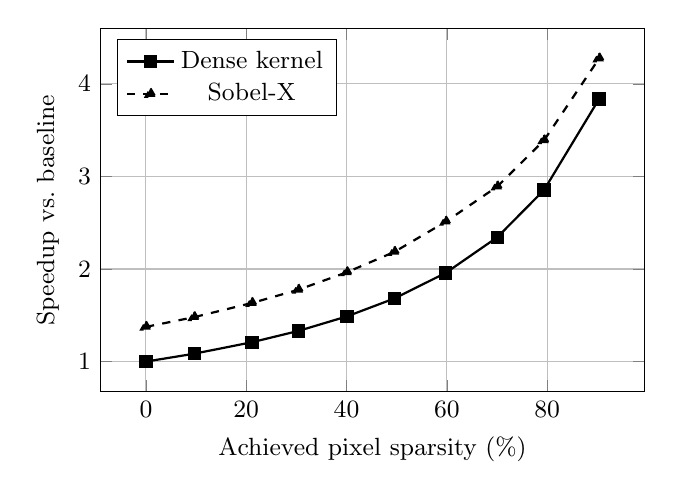
\begin{tikzpicture}
\begin{axis}[width=0.7\textwidth,height=6.2cm,
  xlabel={Achieved pixel sparsity (\%)},ylabel={Speedup vs.\ baseline},
  grid=major,legend pos=north west,legend style={font=\small},
  tick label style={font=\small},label style={font=\small}]
\addplot[mark=square*,thick] coordinates {(0,1.000)(9.62,1.085)(21.14,1.209)(30.39,1.331)(40.08,1.488)(49.55,1.682)(59.79,1.958)(70.06,2.343)(79.38,2.853)(90.37,3.837)};
\addplot[mark=triangle*,thick,dashed] coordinates {(0,1.375)(9.62,1.480)(21.14,1.633)(30.39,1.776)(40.08,1.965)(49.55,2.185)(59.79,2.511)(70.06,2.891)(79.38,3.390)(90.37,4.274)};
\legend{Dense kernel,Sobel-X}
\end{axis}
\end{tikzpicture}
\caption{Measured wall-clock speedup of the ZS engine versus pixel sparsity
(data of Table~\ref{tab:sweep}).}
\label{fig:sweep}
\end{figure}

\subsection{ReLU activation maps with dense kernels}\label{sec:r-relu}
This is the workload on which a static schedule cannot help, because the zeros are
data-dependent. Table~\ref{tab:relu} lists the 14 images. Sparsity is measured on the
activation map before padding, whereas speedups are measured on the zero-padded patches
and therefore include border zeros. Under Rule~2 the speedup ranges from $1.78\times$ to
$4.18\times$ (median $2.01\times$, mean $2.28\times$) at an activation sparsity of
52.8--92.5\,\% (median 61.1\,\%). Under Rule~1 it ranges from $1.66\times$ to $3.71\times$
(median $1.82\times$, mean $2.00\times$). The raw ReLU sparsity before rescaling is
43.7--85.2\,\% (median 52.1\,\%, mean 54.8\,\%). Image I4, a bright flat scene, is an
outlier at the top of both ranges, which is why we report medians. The result depends on
the rescale rule, so both are shown. All 56 workloads had 0 mismatches, and the random
dense kernel gave identical cycle counts to the Gaussian.

\begin{table}[t]
\centering
\caption{ReLU activation maps (dense Gaussian kernel; the random dense kernel gives identical cycle counts). Speedup is the measured wall-clock speedup of the ZS engine over the baseline. I1--I4 are the W1 images and I5--I14 the ten additional images.}
\label{tab:relu}
\small
\setlength{\tabcolsep}{5pt}
\begin{tabular}{lrrrrrrr}
\toprule
 & & \textbf{ReLU} & \multicolumn{2}{c}{\textbf{Rule 2 ($x\gg3$)}} & \multicolumn{2}{c}{\textbf{Rule 1 (max-norm.)}}\\
\textbf{Image} & \textbf{Patches} & \textbf{sparsity} & sparsity & speedup & sparsity & speedup\\
\midrule
I1  & 11{,}648 & 51.64\,\% & 56.40\,\% & 1.867$\times$ & 53.36\,\% & 1.788$\times$\\
I2  & 12{,}288 & 52.14\,\% & 60.16\,\% & 1.988$\times$ & 54.50\,\% & 1.822$\times$\\
I3  &  9{,}216 & 52.32\,\% & 55.89\,\% & 1.859$\times$ & 54.75\,\% & 1.828$\times$\\
I4  & 10{,}880 & 85.24\,\% & 92.52\,\% & 4.183$\times$ & 88.80\,\% & 3.712$\times$\\
I5  & 10{,}880 & 43.69\,\% & 59.16\,\% & 1.950$\times$ & 48.08\,\% & 1.661$\times$\\
I6  & 14{,}976 & 51.98\,\% & 62.02\,\% & 2.048$\times$ & 53.57\,\% & 1.795$\times$\\
I7  & 10{,}880 & 51.41\,\% & 72.17\,\% & 2.465$\times$ & 55.18\,\% & 1.840$\times$\\
I8  &  9{,}216 & 53.97\,\% & 74.39\,\% & 2.583$\times$ & 61.48\,\% & 2.033$\times$\\
I9  & 10{,}880 & 51.32\,\% & 57.64\,\% & 1.910$\times$ & 52.22\,\% & 1.761$\times$\\
I10 & 16{,}384 & 55.07\,\% & 61.95\,\% & 2.039$\times$ & 58.72\,\% & 1.935$\times$\\
I11 & 10{,}880 & 50.69\,\% & 52.81\,\% & 1.778$\times$ & 51.53\,\% & 1.745$\times$\\
I12 & 10{,}880 & 48.53\,\% & 55.16\,\% & 1.832$\times$ & 50.51\,\% & 1.713$\times$\\
I13 & 14{,}208 & 61.92\,\% & 81.64\,\% & 3.039$\times$ & 67.61\,\% & 2.257$\times$\\
I14 & 10{,}880 & 56.65\,\% & 69.70\,\% & 2.361$\times$ & 63.09\,\% & 2.095$\times$\\
\midrule
Total / median & 164{,}096 & 52.06\,\% & 61.05\,\% & 2.014$\times$ & 54.63\,\% & 1.825$\times$\\
\bottomrule
\end{tabular}
\end{table}

\subsection{Ablation: what do OI and CG contribute?}\label{sec:r-ablation}
\emph{Cycles.} The ZS, ZS+OI, ZS+CG, and Combined engines have identical cycle counts on
every patch; so do Baseline, OI, CG, and OI+CG. Neither OI nor CG changes latency.

\emph{Hardware.} ZS+CG and Combined have identical primitive-cell counts (804 cells), as
do CG and OI+CG (721 cells), and each pair has identical post-route LUT and FF counts and
identical worst slack (Table~\ref{tab:res}). The OI logic is removed by synthesis whenever
CG or ZS is present. A reading of the logic that fits this: ZS only dispatches non-zero
operand pairs, so the zero detectors never fire during compute, and with CG a zero
product is never written to the accumulator, so the multiplier output is unobservable.
OI alone costs 21 LUTs at top level (316 versus 295). CG alone uses 15 \emph{fewer} LUTs
than the baseline (280 versus 295); we did not determine why.

\subsection{Resource utilization and timing}\label{sec:r-res}
Table~\ref{tab:res} lists post-route results at 50~MHz; every design uses 0 DSP and 0
BRAM, and every design meets the constraint. Top-level figures include the UART and the
register bank; engine-level figures are the engine hierarchy only. The ZS family needs 56
to 62 more LUTs than the baseline at top level (0.7--0.8\,\% of the 8000 LUTs). Its
estimated frequency is lower than the baseline's (about 71 versus 88~MHz). The baseline
is also free of DSP blocks, so the absence of DSPs does not distinguish the ZS engines.

\begin{table}[t]
\centering
\caption{Post-route resources at 50~MHz (all with 0 DSP and 0 BRAM).}
\label{tab:res}
\small
\setlength{\tabcolsep}{6pt}
\begin{tabular}{lrrrrrr}
\toprule
 & \multicolumn{2}{c}{\textbf{Top}} & \multicolumn{2}{c}{\textbf{Engine}} & \textbf{WNS} & \textbf{Est.\ $F_{\max}$}\\
\textbf{Engine} & LUT & FF & LUT & FF & (ns) & (MHz)\\
\midrule
Baseline     & 295 & 339 & 189 & 80 & 8.620 & 87.9\\
OI           & 316 & 351 & 212 & 88 & 6.757 & 75.5\\
CG           & 280 & 351 & 175 & 88 & 8.181 & 84.6\\
OI+CG        & 280 & 351 & 175 & 88 & 8.181 & 84.6\\
ZS           & 351 & 355 & 247 & 92 & 5.942 & 71.1\\
ZS+OI        & 357 & 355 & 253 & 92 & 5.481 & 68.9\\
ZS+CG        & 352 & 355 & 248 & 92 & 5.995 & 71.4\\
Combined     & 352 & 355 & 248 & 92 & 5.995 & 71.4\\
Static Sobel & 252 & 290 & 155 & 79 & 7.879 & 82.5\\
\bottomrule
\end{tabular}
\end{table}

\subsection{SAIF-based energy estimates}\label{sec:r-energy}
Table~\ref{tab:energy} gives dynamic power and energy per patch for the nine engines on
the W1 stimulus (wrapper v2, zero-delay routed netlists, 44{,}032 patches back-to-back).
All values are tool estimates for engine plus wrapper. ``Harness'' cycles include the two
wrapper cycles, ``engine'' cycles are start to done.

\begin{table}[t]
\centering
\caption{SAIF tool estimates on W1 (Sobel-X, 44{,}032 patches). Harn./Eng.\ = harness/engine cycles per patch; mW = dynamic power. $^{\ast}$\,unresolved (difference below about 5\,\%).}
\label{tab:energy}
\small
\setlength{\tabcolsep}{8pt}
\begin{tabular}{lrrrrr}
\toprule
\textbf{Engine} & \textbf{Harn.} & \textbf{Eng.} & \textbf{mW} & \textbf{nJ/patch} & \textbf{vs.\ base}\\
\midrule
Baseline     & 13.000 & 11.000 & 2.061 & 0.5359 & ref.\\
CG           & 13.000 & 11.000 & 2.024 & 0.5262 & $-1.80\,\%$$^{\ast}$\\
OI+CG        & 13.000 & 11.000 & 2.024 & 0.5262 & $-1.80\,\%$$^{\ast}$\\
OI           & 13.000 & 11.000 & 2.380 & 0.6188 & $+15.48\,\%$\\
ZS           &  9.889 &  7.889 & 2.475 & 0.4895 & $-8.65\,\%$\\
ZS+OI        &  9.889 &  7.889 & 2.495 & 0.4935 & $-7.91\,\%$\\
ZS+CG        &  9.889 &  7.889 & 2.503 & 0.4950 & $-7.62\,\%$\\
Combined     &  9.889 &  7.889 & 2.503 & 0.4950 & $-7.62\,\%$\\
Static Sobel & 10.000 &  8.000 & 1.834 & 0.3668 & $-31.55\,\%$\\
\bottomrule
\end{tabular}
\end{table}

\emph{What is resolved.} OI alone costs $+15.5$\,\% energy per patch. The static Sobel
schedule saves 31.55\,\%, which is far outside the 5\,\% band. ZS saves 7.6--8.7\,\%
depending on variant, only slightly beyond the band, so the sign is believable but the
size is not precise, and the ordering among ZS, ZS+OI, and ZS+CG is unresolved.
\emph{What is not.} CG alone ($-1.80$\,\%) is within the band and we report it as
unresolved. CG and OI+CG, and ZS+CG and Combined, are identical netlists and give
identical numbers, as they should. ZS draws 20 to 21\,\% more instantaneous dynamic power
than the baseline but needs 28\,\% fewer engine cycles, and the energy per patch comes
out lower. The energy per patch includes the two setup cycles of the harness. Static power
(16.383~mW) is the same for every engine and is excluded.

\emph{Dense-kernel ReLU stimulus (W4, Rule~2, Gaussian).} The same four W1 images, with
66.77\,\% zero inputs including border padding, are the stimulus in
Table~\ref{tab:energy2}. On this workload the engine cycles per patch fall from 11 to
4.9905 for ZS, an engine-level speedup of $2.2042\times$ (harness level: $13/6.9905=1.8597\times$). The ZS energy saving of 36.47\,\% is well outside the unresolved band.
ZS+CG shows $-35.35$\,\%, the same within the band as ZS alone. OI again costs
energy ($+16.68$\,\%), and CG alone ($-0.52$\,\%) is unresolved.

\begin{table}[t]
\centering
\caption{SAIF tool estimates on W4 (Rule~2, dense Gaussian kernel, same four images). $^{\ast}$\,unresolved (below about 5\,\%).}
\label{tab:energy2}
\small
\setlength{\tabcolsep}{8pt}
\begin{tabular}{lrrrrr}
\toprule
\textbf{Engine} & \textbf{Harn.} & \textbf{Eng.} & \textbf{mW} & \textbf{nJ/patch} & \textbf{vs.\ base}\\
\midrule
Baseline & 13.000 & 11.000 & 1.157 & 0.3008 & ref.\\
CG       & 13.000 & 11.000 & 1.151 & 0.2993 & $-0.52\,\%$$^{\ast}$\\
OI       & 13.000 & 11.000 & 1.350 & 0.3510 & $+16.68\,\%$\\
ZS       &  6.9905 &  4.9905 & 1.367 & 0.1911 & $-36.47\,\%$\\
ZS+CG    &  6.9905 &  4.9905 & 1.391 & 0.1945 & $-35.35\,\%$\\
\bottomrule
\end{tabular}
\end{table}

\subsection{End-to-end timing over UART}
A request of 18 bytes at 10 bits per byte and 115200 baud takes 1.5625~ms, and request plus
6-byte reply (24 bytes) takes 2.0833~ms per patch. The engine itself needs
$11\cdot20~\mathrm{ns}=220$~ns for the baseline and $7.889\cdot20~\mathrm{ns}=157.8$~ns for ZS on
W1. The engine is therefore busy for roughly 0.008--0.011\,\% of each patch period, and the
board setup is completely UART-bound: end-to-end time will be nearly the same for every
design, with a lower bound of 91.7~s for the 44{,}032 patches of W1. The cycle and energy
differences above apply to back-to-back streaming, not to the board throughput.

\subsection{Hardware-in-the-loop FPGA validation}\label{sec:r-board}
All nine architectural variants were programmed into the physical Spartan-7 SRAM via
Vivado JTAG and validated in hardware on the Invent Logics EDGE board over USB-UART
(115{,}200 baud, 8-N-1 on COM17). Physical validation was conducted across the 3-image
benchmark triad ($33{,}152$ patches per variant: 11{,}648 in I1, 12{,}288 in I2, and
9{,}216 in I3), yielding a total physical workload of $9 \times 33{,}152 = 298{,}368$
physical patch evaluations ($2{,}685{,}312$ physical MAC operations).

Table~\ref{tab:board_master} summarizes the complete board measurements for all nine
variants. Every single run completed with \textbf{0 sum mismatches, 0 cycle count
mismatches, 0 skip count mismatches, and 0 differing pixels} against the golden model
(27 out of 27 runs passed, 100.0\,\% bit-exact).

\begin{table}[t]
\centering
\caption{Physical FPGA hardware validation results on Spartan-7 (XC7S15 @ 50~MHz, 3-image benchmark suite, 33{,}152 patches per engine; 298{,}368 physical patches across all 27 runs). All values are directly measured on physical hardware over UART [BOARD-MEASURED]. $^{\dagger}$In OI, CG, and OI+CG, skips count active low-power gating events on fixed-latency 9-cycle datapaths.}
\label{tab:board_master}
\small
\setlength{\tabcolsep}{4.5pt}
\begin{tabular}{lcrrrrrrcc}
\toprule
\textbf{Architecture} & \textbf{Sel.} & \textbf{Patches} & \textbf{Board Time} & \textbf{Compute Cyc.} & \textbf{Mean Cyc.} & \textbf{Cycles Saved} & \textbf{Cycle Red.} & \textbf{Skips / Gated} & \textbf{Status}\\
\midrule
Baseline        & 0 & 33{,}152 & 533.55~s & 298{,}368 & 9.000 & reference & 0.00\,\% & 0 & \textbf{PASS} (0 err)\\
OI              & 1 & 33{,}152 & 530.43~s & 298{,}368 & 9.000 & 0         & 0.00\,\% & 103{,}234$^{\dagger}$ & \textbf{PASS} (0 err)\\
CG              & 2 & 33{,}152 & 530.46~s & 298{,}368 & 9.000 & 0         & 0.00\,\% & 103{,}234$^{\dagger}$ & \textbf{PASS} (0 err)\\
ZS              & 3 & 33{,}152 & 530.45~s & 195{,}134 & 5.886 & 103{,}234 & 34.60\,\% & 103{,}234 & \textbf{PASS} (0 err)\\
Combined        & 4 & 33{,}152 & 530.92~s & 195{,}134 & 5.886 & 103{,}234 & 34.60\,\% & 103{,}234 & \textbf{PASS} (0 err)\\
ZS+OI           & 5 & 33{,}152 & 530.55~s & 195{,}134 & 5.886 & 103{,}234 & 34.60\,\% & 103{,}234 & \textbf{PASS} (0 err)\\
ZS+CG           & 6 & 33{,}152 & 530.42~s & 195{,}134 & 5.886 & 103{,}234 & 34.60\,\% & 103{,}234 & \textbf{PASS} (0 err)\\
OI+CG           & 7 & 33{,}152 & 531.05~s & 298{,}368 & 9.000 & 0         & 0.00\,\% & 103{,}234$^{\dagger}$ & \textbf{PASS} (0 err)\\
Static Sobel    & 8 & 33{,}152 & 532.06~s & 198{,}912 & 6.000 &  99{,}456 & 33.33\,\% & 0 & \textbf{PASS} (0 err)\\
\midrule
\textbf{Total / All 27 Runs} & -- & \textbf{298{,}368} & \textbf{4{,}779.89~s} & \textbf{2{,}076{,}826} & -- & \textbf{512{,}392} & -- & \textbf{722{,}638} & \textbf{27/27 PASS}\\
\bottomrule
\end{tabular}
\end{table}

\emph{Key hardware findings.}
\begin{enumerate}
\item \emph{Compute cycle reduction:} On physical hardware, the four ZS engines (ZS, ZS+OI,
ZS+CG, Combined) require exactly 195{,}134 compute cycles across the triad (mean 5.886
cycles/patch), compared to 298{,}368 cycles for the baseline (mean 9.000 cycles/patch).
This represents an exact **34.60\,\% compute-cycle reduction** (103{,}234 cycles saved per
triad run), confirming the cycle model on real FPGA hardware.
\item \emph{Fixed-schedule architectures:} Baseline, OI, CG, and OI+CG operate at exactly
9.000 cycles/patch on every run. For OI, CG, and OI+CG, the hardware reports exactly 103{,}234
gating events across the triad (36{,}396 in I1, 38{,}136 in I2, and 28{,}702 in I3).
In these engines, the datapath remains active for 9 cycles, but operand inputs are
clamped to zero or accumulator registers are clock-enable disabled during the 103{,}234
detected zero intervals.
\item \emph{Static Sobel engine:} The static engine executed in exactly 198{,}912 compute
cycles (6.000 cycles/patch, 33.33\,\% cycle reduction vs.\ baseline) with zero skips
reported, consistent with the synthesis removal of the three zero-weight taps.
\item \emph{Inter-variant counter consistency:} On physical hardware, ZS, ZS+OI, ZS+CG,
and Combined produced strictly identical compute cycle counts (68{,}436 for I1, 72{,}456
for I2, 54{,}242 for I3) and skip counts (36{,}396 for I1, 38{,}136 for I2, 28{,}702 for
I3). Similarly, OI, CG, and OI+CG matched each other exactly in gating event counts.
\item \emph{Throughput bound by UART:} As predicted in Section~\ref{sec:r-sobel}, the
total host execution time per triad was 530.42~s to 533.55~s across all nine designs
(average throughput 62.17 to 62.50 patches/s). The compute time accounts for less than
0.01\,\% of the patch interval; UART framing completely governs the elapsed time in this
host-in-the-loop configuration.
\item \emph{No energy claims from board data:} The FPGA hardware reply carries the 32-bit
integer sum, an 8-bit compute cycle counter, and an 8-bit skip counter. No physical power
measurement was instrumented on the board, and no power or energy claim is derived from
the hardware measurements.
\end{enumerate}

\begin{figure}[t]
\centering
\begin{minipage}{0.31\textwidth}
  \centering
  \figorbox{results/paper_assets/comparison_image1_composite.png}{\linewidth}{Image 1: Input vs FPGA output}
  \centerline{\small (a) Workload 1: \texttt{image1.jpg}}
\end{minipage}\hfill
\begin{minipage}{0.31\textwidth}
  \centering
  \figorbox{results/paper_assets/comparison_image2_composite.png}{\linewidth}{Image 2: Input vs FPGA output}
  \centerline{\small (b) Workload 2: \texttt{image2.jpg}}
\end{minipage}\hfill
\begin{minipage}{0.31\textwidth}
  \centering
  \figorbox{results/paper_assets/comparison_image3_composite.png}{\linewidth}{Image 3: Input vs FPGA output}
  \centerline{\small (c) Workload 3: \texttt{image3.jpg}}
\end{minipage}
\caption{Visual validation of physical FPGA edge detection across the three benchmark workloads. In each pair, the left panel is the original grayscale input image and the right panel is the reconstructed edge map generated from 32-bit sums produced on the Spartan-7 FPGA. Pixel-by-pixel subtraction between baseline and all low-power variants yielded zero differing pixels ($\Delta = 0$).}
\label{fig:board_images}
\end{figure}

% =============================================================================
\section{Discussion and Limitations}\label{sec:disc}
\textbf{Where the benefit comes from.} On Sobel-X, nearly all of the saving is the
kernel's three structural zeros, which a static schedule exploits with 155 engine LUTs
and no detection logic, and which also gave it the lowest energy estimate among the nine
engines (31.55\,\% below the baseline). Run-time detection earns its extra area where the
zeros depend on the data: on ReLU activation maps with dense kernels it was
$1.78\times$--$4.18\times$ faster, never slower than the baseline even on fully dense
patches, and the estimated energy per patch fell by 36.5\,\%. The summary is that
ZS is a general sparsity engine whose strength is dense-kernel workloads, and the static
schedule is the better choice when the kernel is fixed and known.

\textbf{What OI and CG did.} OI added logic and energy when used alone and disappeared
from the hardware when combined with CG or ZS. CG alone changed the estimate by less
than our noise band and is unresolved. We did not determine why CG alone uses fewer LUTs
than the baseline.

\textbf{Limitations.}
(i)~Physical FPGA validation verified functional equivalence and cycle counts over UART,
but the board setup was not instrumented for physical power rail measurement; all energy
figures remain tool estimates from zero-delay routed netlists.
(ii)~Energy figures are SAIF tool estimates for engine plus wrapper on one device, from
zero-delay netlists (without glitch power); no physical power measurement was made and
none is claimed from board data.
(iii)~Differences below about 5\,\% are unresolved; the 5\,\% figure comes from two
baseline netlists in an earlier flow and was not repeated in the final flow, and the
sensitivity to the order of the input images was checked only in that earlier flow.
(iv)~The 17 mismatches observed in SDF-annotated gate-level simulation of image~3 were
proven on physical hardware to be simulation model artifacts (Section~\ref{sec:r-board}),
confirming that the physical logic is free of timing errors at 50~MHz.
(v)~Estimated $F_{\max}$ values are derived from slack at 50~MHz.
(vi)~The ReLU maps come from a Sobel layer with an arbitrary rescale, not from a trained
CNN, and the static schedule applies to Sobel-X only.
(vii)~The ten additional images are of unknown provenance until documented.
(viii)~We do not know why CG alone has fewer LUTs than the baseline.
(ix)~The design streams patches over UART; an on-chip line buffer would be needed to feed
the engine from a frame at full rate, which we have not built.

% =============================================================================
\section{Conclusion}\label{sec:concl}
A serial 3$\times$3 engine with priority-encoded zero-skipping reduced the measured
compute latency on Sobel-X filtering of real images from 9.00 to 5.886 cycles per
patch (a 34.60\,\% cycle reduction), at a cost of 56 to 62 LUTs, and matched a golden
model exactly in RTL simulation, zero-delay gate-level netlists, and physical FPGA
hardware validation across 298{,}368 patches on a Spartan-7 XC7S15 FPGA. Almost all of
that gain on Sobel is explained by the kernel's own zeros, which a static six-tap schedule
exploits (33.33\,\% cycle reduction) with less logic and, in our SAIF tool estimate,
31.6\,\% lower energy per patch. On data-dependent sparsity, namely ReLU feature maps
with dense kernels, the ZS engine was $1.78\times$ to $4.18\times$ faster (median
$2.01\times$), was never slower than the baseline, and its estimated energy per patch
was 36.5\,\% lower. Operand isolation contributed nothing in the implemented hardware,
and CE gating alone was within the unresolved band. Physical FPGA validation resolved
the 17 prior SDF simulation anomalies as simulator modeling artifacts. Future work
includes physical board-level power measurements using a calibrated current-sense monitor,
evaluation on activations from a trained neural network, and an on-chip BRAM line buffer.

% =============================================================================
% References are numbered in order of first citation in the text.
\begin{thebibliography}{20}
\bibitem{horowitz2014} M.~Horowitz, ``Computing's energy problem (and what we can do about it),'' in \emph{ISSCC Dig. Tech. Papers}, 2014, pp. 10--14.
\bibitem{sze2017} V.~Sze, Y.-H. Chen, T.-J. Yang, and J.~S. Emer, ``Efficient processing of deep neural networks: A tutorial and survey,'' \emph{Proc. IEEE}, vol.~105, no.~12, pp. 2295--2329, Dec. 2017.
\bibitem{han2015} S.~Han, J.~Pool, J.~Tran, and W.~J. Dally, ``Learning both weights and connections for efficient neural networks,'' in \emph{Advances in Neural Information Processing Systems 28}, 2015, pp. 1135--1143. % VERIFY page range (found on mlanthology.org only)
\bibitem{eyeriss2017} Y.-H. Chen, T.~Krishna, J.~S. Emer, and V.~Sze, ``Eyeriss: An energy-efficient reconfigurable accelerator for deep convolutional neural networks,'' \emph{IEEE J. Solid-State Circuits}, vol.~52, no.~1, pp. 127--138, Jan. 2017. % VERIFY that the zero-input gating statement in Sec. II matches the paper text
\bibitem{eie2016} S.~Han, X.~Liu, H.~Mao, J.~Pu, A.~Pedram, M.~A. Horowitz, and W.~J. Dally, ``EIE: Efficient inference engine on compressed deep neural network,'' in \emph{Proc. ISCA}, 2016, pp. 243--254.
\bibitem{cnvlutin2016} J.~Albericio, P.~Judd, T.~Hetherington, T.~Aamodt, N.~E. Jerger, and A.~Moshovos, ``Cnvlutin: Ineffectual-neuron-free deep neural network computing,'' in \emph{Proc. ISCA}, 2016, pp. 1--13.
\bibitem{scnn2017} A.~Parashar \emph{et al.}, ``SCNN: An accelerator for compressed-sparse convolutional neural networks,'' in \emph{Proc. ISCA}, 2017, pp. 27--40.
\bibitem{nullhop2019} A.~Aimar \emph{et al.}, ``NullHop: A flexible convolutional neural network accelerator based on sparse representations of feature maps,'' \emph{IEEE Trans. Neural Netw. Learn. Syst.}, vol.~30, no.~3, pp. 644--656, Mar. 2019.
\bibitem{vestias2019} M.~P. V\'estias, R.~P. Duarte, J.~T. de~Sousa, and H.~C. Neto, ``Fast convolutional neural networks in low density FPGAs using zero-skipping and weight pruning,'' \emph{Electronics}, vol.~8, no.~11, art.~1321, 2019.
\bibitem{munch2000} M.~M{\"u}nch, B.~Wurth, R.~Mehra, J.~Sproch, and N.~Wehn, ``Automating RT-level operand isolation to minimize power consumption in datapaths,'' in \emph{Proc. DATE}, 2000, pp. 624--631.
\bibitem{wu2000} Q.~Wu, M.~Pedram, and X.~Wu, ``Clock-gating and its application to low power design of sequential circuits,'' \emph{IEEE Trans. Circuits Syst. I}, vol.~47, no.~3, pp. 415--420, Mar. 2000.
\bibitem{tpu2017} N.~P. Jouppi \emph{et al.}, ``In-datacenter performance analysis of a tensor processing unit,'' in \emph{Proc. ISCA}, 2017, pp. 1--12.
\bibitem{deepcomp2016} S.~Han, H.~Mao, and W.~J. Dally, ``Deep compression: Compressing deep neural networks with pruning, trained quantization and Huffman coding,'' in \emph{Proc. ICLR}, 2016.
\bibitem{jacob2018} B.~Jacob \emph{et al.}, ``Quantization and training of neural networks for efficient integer-arithmetic-only inference,'' in \emph{Proc. IEEE/CVF CVPR}, 2018, pp. 2704--2713.
\bibitem{cambriconx2016} S.~Zhang \emph{et al.}, ``Cambricon-X: An accelerator for sparse neural networks,'' in \emph{Proc. IEEE/ACM MICRO}, 2016, pp. 1--12.
\bibitem{sparten2019} A.~Gondimalla, N.~Chesnut, M.~Thottethodi, and T.~N. Vijaykumar, ``SparTen: A sparse tensor accelerator for convolutional neural networks,'' in \emph{Proc. IEEE/ACM MICRO}, 2019, pp. 151--165.
\bibitem{zhang2015} C.~Zhang, P.~Li, G.~Sun, Y.~Guan, B.~Xiao, and J.~Cong, ``Optimizing FPGA-based accelerator design for deep convolutional neural networks,'' in \emph{Proc. ACM/SIGDA Int. Symp. FPGA}, 2015, pp. 161--170.
\bibitem{kitayama2021} A.~Kitayama \emph{et al.}, ``Low-power implementation techniques for convolutional neural networks using precise and active skipping methods,'' \emph{IEICE Trans. Electron.}, vol.~E104-C, no.~7, pp. 330--337, Jul. 2021. % VERIFY author list
\bibitem{hoang2010} T.~T. Hoang, M.~Sj{\"a}lander, and P.~Larsson-Edefors, ``A high-speed, energy-efficient two-cycle multiply-accumulate (MAC) architecture and its application to a double-throughput MAC unit,'' \emph{IEEE Trans. Circuits Syst. I}, vol.~57, no.~12, pp. 3073--3081, Dec. 2010.
\bibitem{ug907} AMD (Xilinx), ``Vivado Design Suite User Guide: Power Analysis and Optimization,'' UG907, v2025.2, Nov. 2025. % VERIFY: use the UG907 version that matches Vivado v2026.1 once it is available
\end{thebibliography}

\end{document}
